\setcounter{chapter}{5}
\chapter{\acs{fastPLI}}
\label{chap:Software}
% 
\cleanchapterquote{There are only two kinds of languages: the ones people complain about and the ones nobody uses.}{Bjarne Stroustrup}{The \cpp{} Programming Language}
% 
% 
\includegraphics[width=.075\textwidth]{gfx/Scihub_raven.png}
% \cleanchapterquote{Journal paywalls are an example of something that works in the reverse direction, making communication less open and efficient.}{Alexandra Elbakyan}{}
% % 
% % \tikz[remember picture,overlay] \node[inner sep=0pt] at (0,0){
\includegraphics[height=7em]{gfx/Scihub_raven.png}};
% % \hspace{-10em}
% % \clearpage opacity=0.3,
% 
% 
%  
\section{Introduction}
% 
In the previous chapters, the algorithms for creating dense \ac{WM} fiber models (see \cref{chap:sof:modeling}) and simulating \ac{3D-PLI} (see \cref{cha:sof:simulation}) are described.
Both algorithms are designed to work without knowledge of the other.
This allows \eg{} to be useful for models in other domains, such as \ac{dMRI} (\cite{Ginsburger2019,ginsburgerDis2019}).
However, in addition to providing algorithms that are intended to be very fast and thus as in this case at a very low level, it is also necessary to provide an \ac{API} that provides an interface to the user.
This interface must be designed in such a way that the user has a good experience when working with the algorithms.
Among other things, this means a high level of abstraction with logical and easy-to-use naming systems.
A high level of abstraction in software design means that unnecessary systems and generalizations of functionalities are hidden.
% 
\par
% 
In addition, the algorithms should be accessible to a wide audience.
Among other things, this means that the program must be installable and easy to understand, even if no programming knowledge is available.
The latter is of course a problem, however, in the last decades more and more higher programming languages have been designed to be easily understandable.
% 
\par
% 
For the above reasons, the \python{} programming language was chosen.
It has become increasingly popular in the last decade, especially in data science.
The core algorithms remain in \cpp{} as described in their chapters to ensure efficiency, speed and parallelization.
%
\section{Toolbox}
% 
\begin{figure}[!ht]
\centering
% \resizebox{0.95\textwidth}{!}{
% \setlength{\tikzwidth}{0.75\textwidth}
\inputtikz{gfx/fastpli/fastpli_pipeline}
% }
\caption[\acs{fastPLI}]{\ac{fastPLI} package structure}
\label{fig:fastpli}
\end{figure}
% 
The \python{} package is called \ac{fastPLI}.
Its source code is publicly available and \cite{fastpli,Matuschke2021} published.
The software package includes functionalities for the analysis and visualization of the nerve fiber models as well as for the analysis of the simulation analogous to the current routine experimental measurements, \eg{} inclination analysis.
% 
% 
% 
\subsection{Documentation}
% 
\begin{figure}[!t]
    \centering
    \resizebox{\textwidth}{!}{\fbox{
    \begin{tabular}{c|c}
    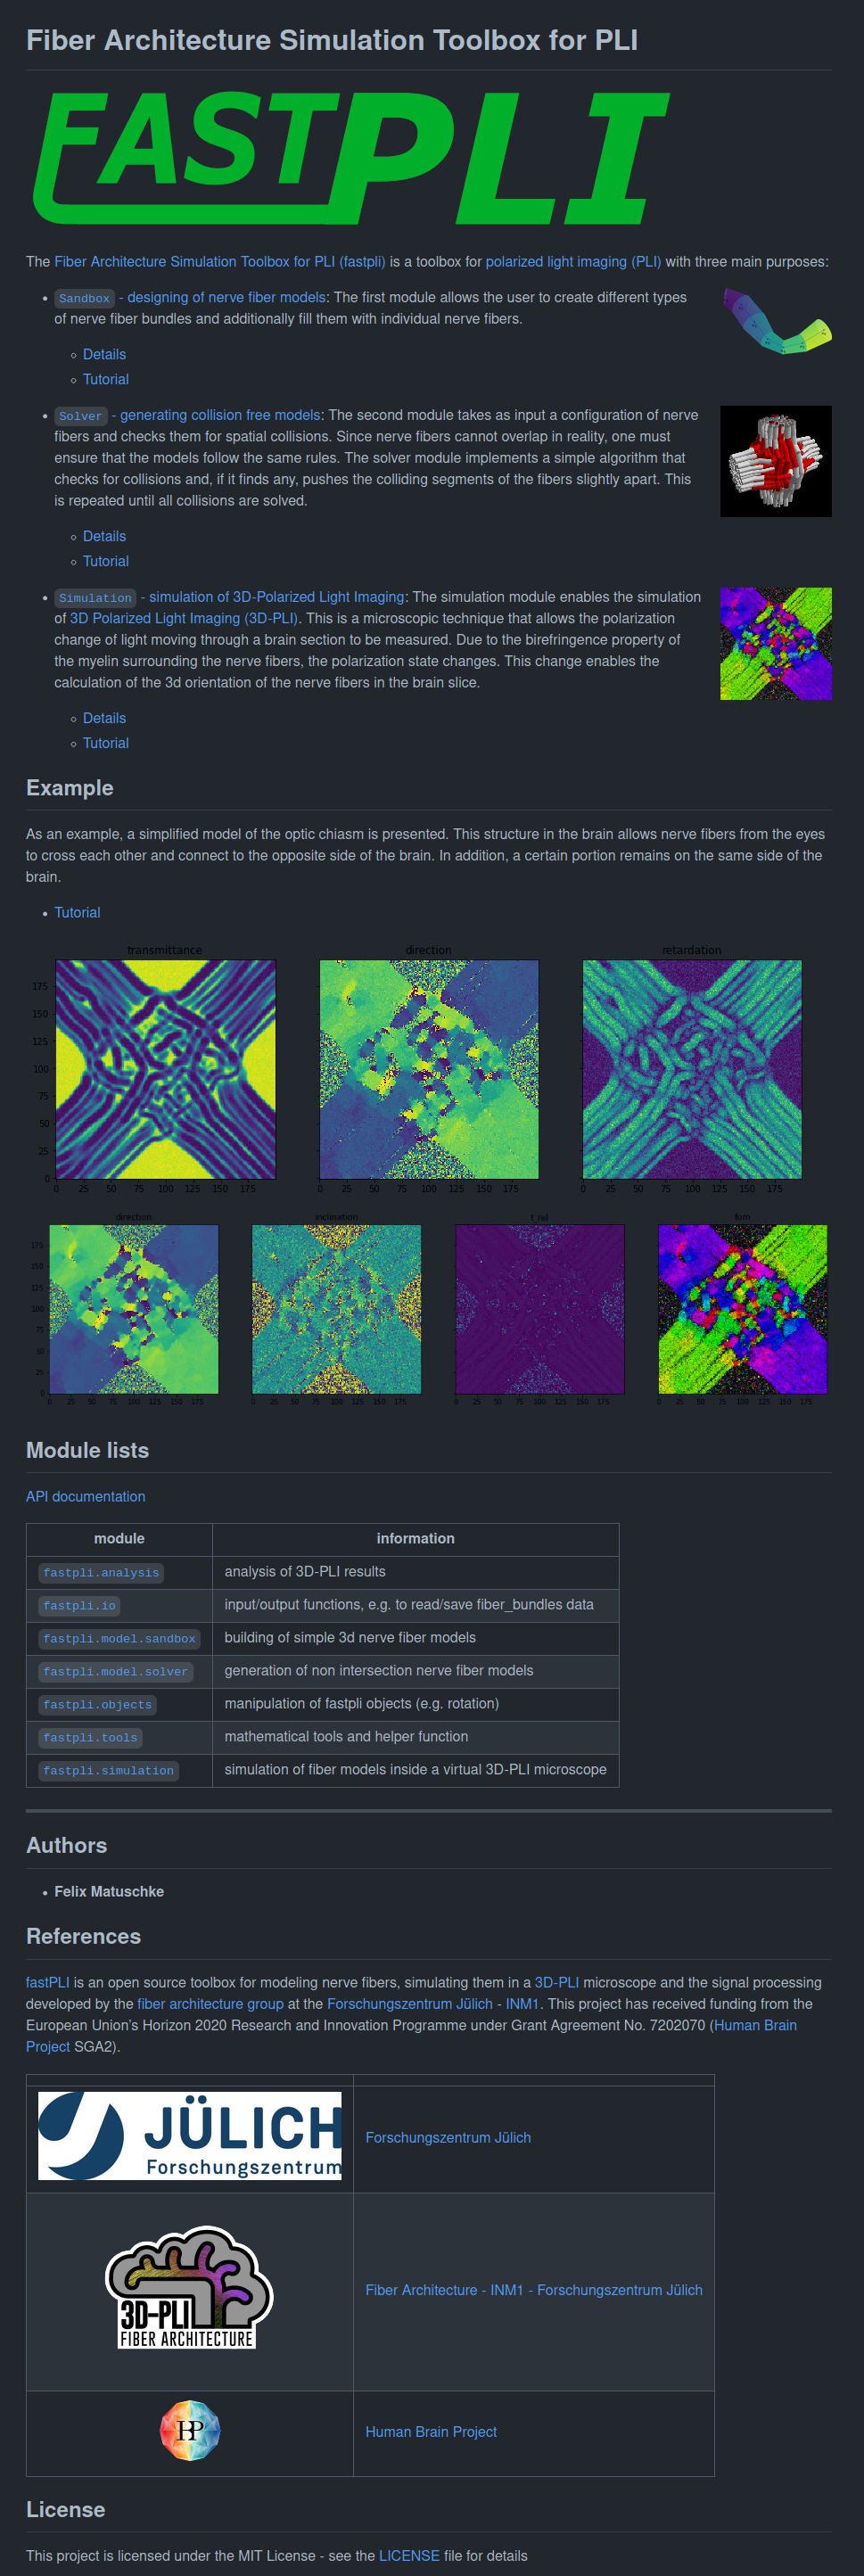
\includegraphics[valign=T,trim=0 1300 0 0, clip]{gfx/fastpli/fastpli_wiki.png} &
 	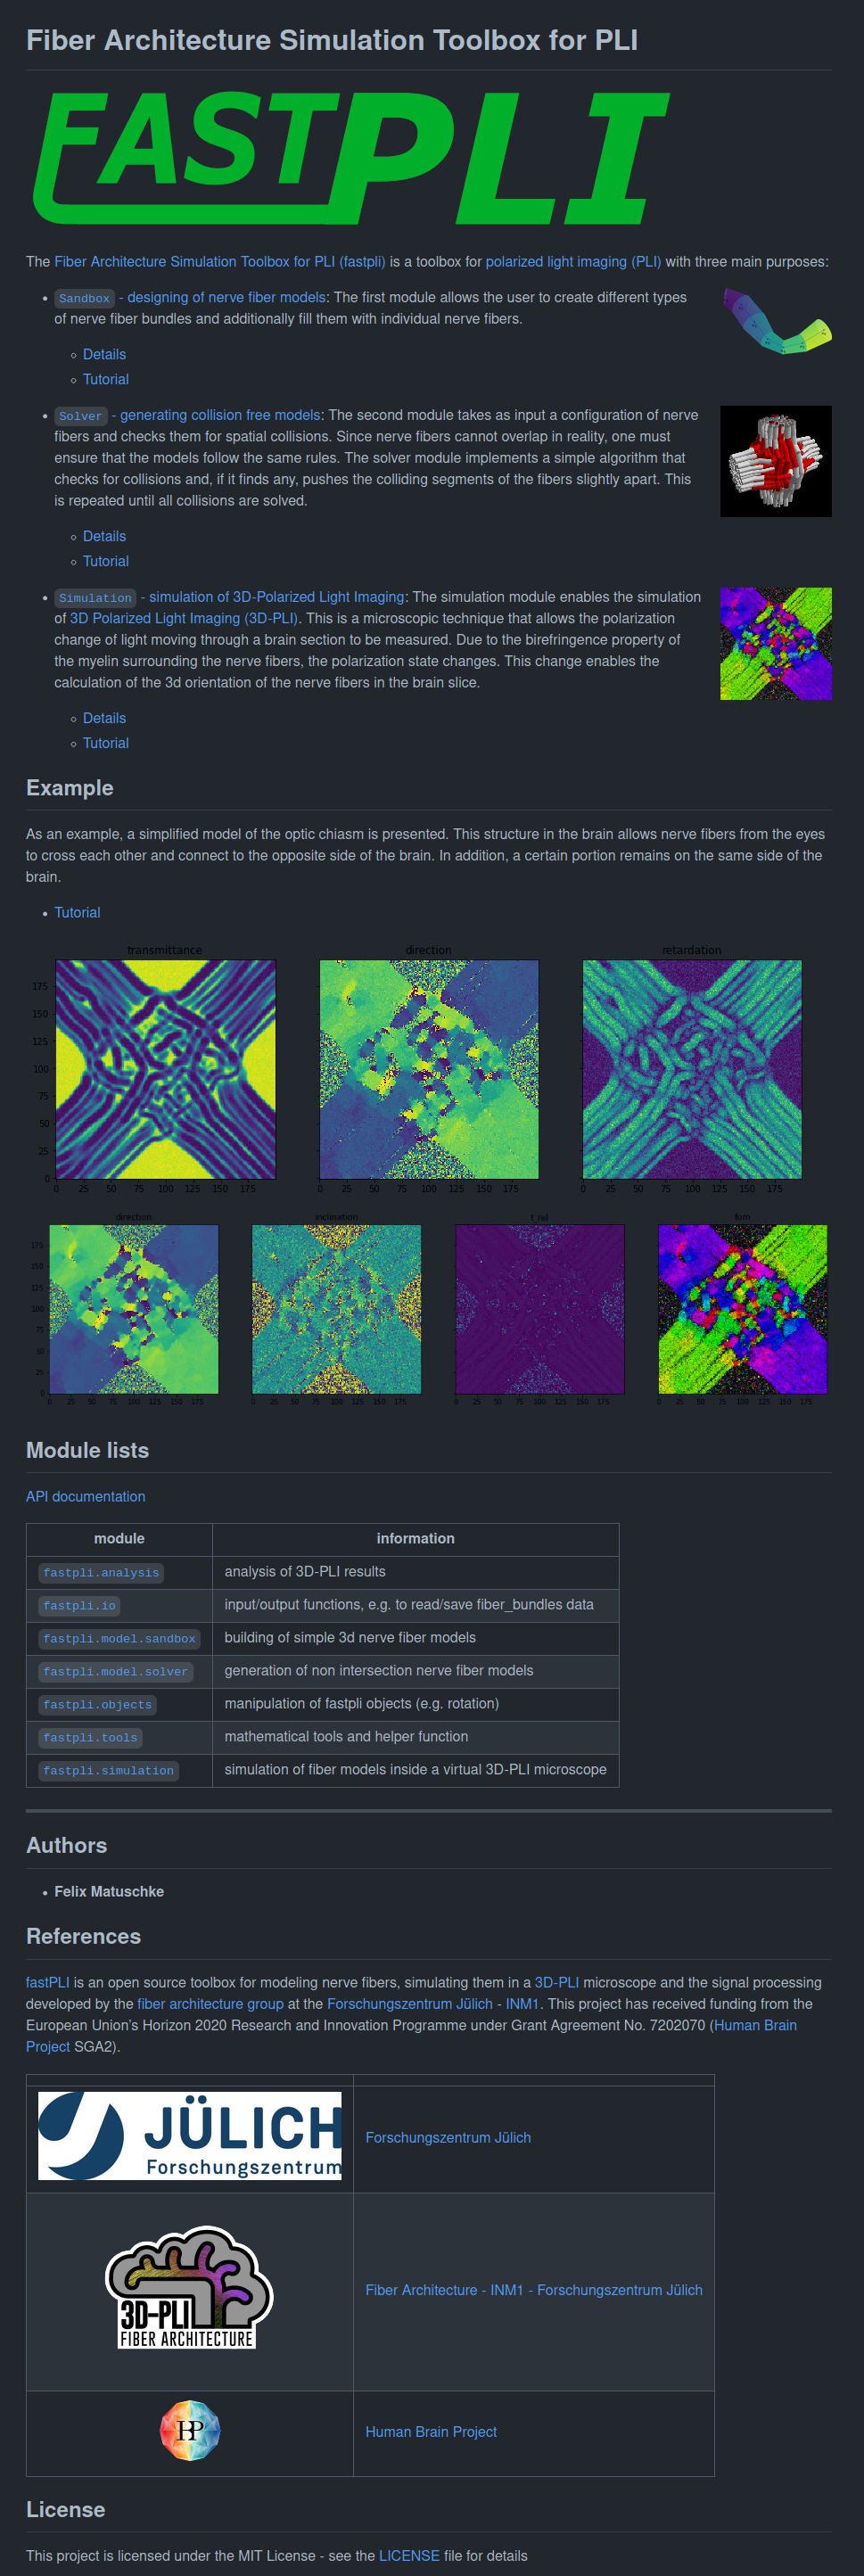
\includegraphics[valign=T,trim=0 0 0 1580, clip]{gfx/fastpli/fastpli_wiki.png} \\
    \end{tabular}
    }}
	\caption[Documentation]{Documentation Wiki Page of the Github repository \url{https://github.com/3d-pli/fastpli/wiki}.}
	\label{fig:fastpli_wiki}
\end{figure}
% 
As is common in software development, all methods are provided with docstrings (documentation string) to help the user understand how they work.
These are displayed e.g. by modern editors automatically wäres during programming, in order to give assistance.
These docstrings are also used for an automatic release of a \ac{API} documentation\footnote{\url{https://3d-pli.github.io/fastpli/}}.
In addition, a wiki page (see \cref{fig:fastpli_wiki}) describing the main features is available, which is an essential part of the review process for publication in \textit{the Journal of Open Source Software (JOSS)} \cite{Matuschke2021} \footnote{review openly accessible at \url{https://github.com/openjournals/joss-reviews/issues/3042}}.
To help users get started quickly, both executable \python{} scripts and Jupyter notebooks are available as tutorials.
A combined example for the whole package based on the optical chiasm\footnote{the nerve fiber crossing of the optical path from eyes to occipital lobe} is accessible as the last part.
% 
% 
% 
\subsection{Dependencies}
% 
\paragraph{Python:}
\begin{description}
\item[numpy:] Base N-dimensional array package \cite{2019arXiv190710121V}\\
\url{https://numpy.org/}
\item[scipy:] Fundamental library for scientific computing \cite{2019arXiv190710121V}\\
\url{https://www.scipy.org/} 
\item[numba:] Acceleration of Python Functions \cite{Lam2015}\\
\url{https://numba.pydata.org/}
\item[mpi4py:] MPI for Python \cite{Dalcn2005, Dalcn2008, Dalcin2011}\\
\url{https://bitbucket.org/mpi4py/mpi4py/src/master/}
\item[h5py:] HDF5 for Python \cite{collette_python_hdf5_2014, hdf5}\\
\url{https://www.h5py.org/}
\end{description}
% 
\paragraph{C++:}
\begin{description}
\item[MPI:] Message Passing Interface \cite{message2015mpi}\\
\url{https://www.mpi-forum.org/}
\item[OpenMP:] Open Multi-Processing, API for multi-platform shared memory multiprocessing programming \cite{dagum1998openmp}\\
\url{https://www.openmp.org/}
\item[OpenGL:] Open Graphics Library \cite{khronos}\\
\url{www.opengl.org}
\item[Pybind11:] Seamless operability between C++11 and Python \cite{pybind11}\\ \url{https://github.com/pybind/pybind11} 
\end{description}
%
% 
At this point, only Linux builds are supported.
However, for current Windows versions, the \ac{WSL} provides a fully functional Linux kernel inside Windows.
This makes it possible to run the same software as under native linux distributions.
Current macOS versions are not supported, but due to the minimalistic style of the \ac{fastPLI} package, the required changes should be feasible with minimal modifications.
% 
% 
\subsection{Tests/Verification/...}
% 
To provide fully tested software, each module with its main methods is automatically tested after each push\footnote{uploud of an \textit{git} commit} with a Github action\footnote{they are commenly used for automatic build, test and deployment of the software and documentation}. tested.
This action runs the two latest Ubuntu Long Term Support versions (18.04 LTS and 20.04 LTS) and the most commonly used Python3 versions (3.6 and 3.8) to provide a wide range of supported common versions.
In addition, the \textit{Github actions} run all test scripts, check tutorial files, check code format and linting for consistency, and publish the latest documentation.
% 
% 
% 
\par
\noindent\rule{\textwidth}{2pt}
\newpage
%
%  
% 
%  
\section{modules}
% 
\begin{lstfloat}[!ht]
\lstset{style=python}
\begin{lstlisting}
import fastpli
''' __version__
'''

import fastpli.analysis
''' affine_transformation
    epa
    images
    rofl
'''

import fastpli.io
''' fiber_bundles
'''

import fastpli.model.sandbox
''' fill
    shape
'''

import fastpli.model.solver
''' class Solver
    __solver.cpython.so
    _solver.py
'''

import fastpli.objects
''' fiber
    fiber_bundle
    fiber_bundles
'''

import fastpli.simulation
''' class Simpli
    __generation.cpython.so
    __simulation.cpython.so
    _simpli.py
    optic
'''

import fastpli.tools
''' label_converter
    rotation
'''
\end{lstlisting}
\caption[Overview \fastpli{} package]{Overview \fastpli{} package with containing modules}
% 	\label{alg:simulation}
\end{lstfloat}
% 
% 
%  
\subsection{fastpli.analysis}
\begin{lstfloat}[!ht]
\lstset{style=python}
\begin{lstlisting}
import fastpli.analysis
fastpli.analysis.affine_transformation
    # apply affine transformations to images (e.g. untilt)
fastpli.analysis.epa
    # analysis of 2d PLI images
fastpli.analysis.images
    # analysis/generation of color images (FOM, VectorImages, ...)
fastpli.analysis.rofl
    # analysis tilted PLI images
\end{lstlisting}
\caption{\code{fastpli.analysis}}
% 	\label{alg:simulation}
\end{lstfloat}
% 
% 
%  
\subsection{fastpli.io}
\begin{lstfloat}[!ht]
\lstset{style=python}
\begin{lstlisting}
import fastpli.io
fastpli.io.fiber_bundles
    # io operations for dat-files and hdf5-files
    # for the fiber_bundles format.
\end{lstlisting}
\caption{\code{fastpli.io}}\label{alg:fastpli.io}
\end{lstfloat}
% 
\paragraph{fiber\_bundles.py} contains io routines (see \cref{alg:fastpli.io}) for reading and saving fiber\_bundles into dat-files or hdf5-files. dat-files are text files which have to following structure as in \cref{alg:dat-file}. This dataformat is used to be as exchange friendly as possible for new users. \hdf{} files on the other hand are a binary dataformat \cite{hdf5}, where the individual datasets are arange in datacontainers, like the file explorer (see \cref{alg:hdf5}). The data contains 4d arrays, which are explained in \cref{sec:nerve_fiber_representation}.
% 
\begin{lstfloat}[!ht]
\lstset{style=common,morecomment=[l][\color{syntax_green}]{<-},}
\begin{lstlisting}
-6.55 -18.93 -64.98 3.75 <- x y z r
-5.73 -14.89 -63.37 3.4
-4.42 -13.66 -58.95 3.05
    <- empty line indicates new fiber
-1.96 -10.07 -52.5 2.92
-1.03 -9.4 -48.62 2.93

    <- two empty lines indicates new fiber bundle
3.4 -4.02 -44.76 3.11
6.22 -1.04 -42.45 3.26
\end{lstlisting}
\caption{exemplary dat-file format. Commets are currently not allowed and are only for the readers eyes.}\label{alg:dat-file}
\end{lstfloat}
% 
\begin{lstfloat}[!ht]
\lstset{style=common}
\begin{lstlisting}
GROUP "/" { # fiber_bundles path
  GROUP "0" { # id of fiber_bundle
      DATASET "0" { # id of fiber
         DATATYPE  H5T_IEEE_F64LE
         DATASPACE  SIMPLE { ( 3, 4 ) / ( 3, 4 ) }
         DATA {
         (0,0): -6.55, -18.93, -64.98, 3.75,
         (1,0): -5.73, -14.89, -63.37, 3.4,
         (2,0): -4.42, -13.66, -58.95, 3.05,
         }
      }
      DATASET "1" { # id of fiber
         DATATYPE  H5T_IEEE_F64LE
         DATASPACE  SIMPLE { ( 2, 4 ) / ( 2, 4 ) }
         DATA {
         (3,0): -1.96, -10.07, -52.5, 2.92,
         (4,0): -1.03, -9.4, -48.62, 2.93,
         }
      }
  }
  GROUP "1" { # id of fiber_bundle
      DATASET "0" { # id of fiber
         DATATYPE  H5T_IEEE_F64LE
         DATASPACE  SIMPLE { ( 2, 4 ) / ( 2, 4 ) }
         DATA {
         (0,0): 3.4, -4.02, -44.76, 3.11,
         (1,0): 6.22, -1.04, -42.45, 3.26,
         }
      }
  }
}
\end{lstlisting}
\caption{exemplary hdf5-file format.} \label{alg:hdf5}
\end{lstfloat}
% 
% 
% 
\subsection{fastpli.model.sandbox}
\begin{lstfloat}[!ht]
\lstset{style=python}
\begin{lstlisting}
import fastpli.model.sandbox
fastpli.model.sandbox.fill
    # filling of trajectaries with seed points as fiber_bundles
fastpli.model.sandbox.build
    # building of geometries
\end{lstlisting}
\caption{\code{fastpli.model.sandbox}}
% 	\label{alg:simulation}
\end{lstfloat}
% 
% 
% 
\subsection{fastpli.model.solver}
\begin{lstfloat}[!ht]
\lstset{style=python}
\begin{lstlisting}
import fastpli.model.solver
fastpli.model.solver.Solver
    # Class wrapper for C++ class.
    # Solves any 3d configurations of fibers to a non colliding ...
\end{lstlisting}
\caption{\code{fastpli.model.solver}}
% 	\label{alg:simulation}
\end{lstfloat}
% 
% 
% 
\subsection{fastpli.simulation}
\begin{lstfloat}[!ht]
\lstset{style=python}
\begin{lstlisting}
import fastpli.simulation
fastpli.simulation.Simpli
    # Class wrapper for C++ class.
    # Generatoes:
    #   - discretisied Tissue Volume
    #   - 3D PLI images
    #   - analysis of resultss
\end{lstlisting}
\caption{\code{fastpli.simulation}}
% 	\label{alg:simulation}
\end{lstfloat}
% 
% 
% 
\subsection{fastpli.tools}
\begin{lstfloat}[!ht]
\lstset{style=python}
\begin{lstlisting}
import fastpli.tools
fastpli.tools.label_converter
    # conversion of discretisied tissue to 
    # maxwell-solver input format
fastpli.tools.rotation
    # rotation matricies for 3d rotaions
\end{lstlisting}
\caption{\code{fastpli.tools}}
% 	\label{alg:simulation}
\end{lstfloat}
% 
% 
% 
